\providecommand{\main}{..}
\documentclass[\main/ApuntesPL.tex]{subfiles}

% !TEX root = ../ApuntesPL.tex

\begin{document}
  \begin{tikzpicture}
    \node[rectangle, draw = black, align = center, rectangle split, rectangle split horizontal, rectangle split parts = 2] (cl1) {};
    \node[rectangle, draw = black, right = .2 of cl1, align = center, rectangle split, rectangle split horizontal, rectangle split parts = 2] (cl2) {};
    \node[rectangle, draw = black, right = .2 of cl2, align = center, rectangle split, rectangle split horizontal, rectangle split parts = 2] (cl3) {};

    \node[unit, right = of cl3, align = center] (ansi) {Analizador\\sintáctico};
    \node[err, below=of ansi] (err) {error};

    \node[rectangle, right=2of ansi, label={Árbol incontextual}] (t1) {$e_0$};
    \node[rectangle, below left =.5 of t1] (t2) {$e_1$};
    \node[rectangle, below right =.5 of t1] (t3) {$e_2$};
    \node[rectangle, below left =.5 of t3] (t4) {$e_3$};
    \node[rectangle, below right =.5 of t3] (t5) {$e_4$};
    \node[rectangle, below left =.5 of t4] (t6) {$e_5$};
    \node[rectangle, below right =.5 of t4] (t7) {$e_6$};
    \node[rectangle, below left =.5 of t7] (t8) {$e_7$};
    \node[rectangle, below right =.5 of t7] (t9) {$e_8$};

    \draw[myarrow] (cl3.east) -- ++(0,0) -> (ansi.west);
    \draw[myarrow] (ansi.south) -- ++(0,0) -> (err.north);
    \draw[myarrow] (ansi.east) -- ++(0,0) -> (t1.west);

    \path[thick]
      (t1.south)  edge (t2)
                  edge (t3)
      (t3.south)  edge (t4)
                  edge (t5)
      (t4.south)  edge (t6)
                  edge (t7)
      (t7.south)  edge (t8)
                  edge (t9);
  \end{tikzpicture}

  \bigskip
  \par
  Hipótesis: Las cadenas de clases léxicas generadas por el analizador léxico forman un lenguaje incontextual.

  \section{Recordatorio}
    \subsection{Gramática}
      Sea una GI (Gramática Incontextual), GI(N,T,P,S):
      \begin{itemize}
        \item N $\equiv$ alfabeto de no terminales $\Rightarrow$ clases sintácticas.
        \item T $\equiv$ alfabeto de terminales $\Rightarrow$ clases léxicas.
        \item P $\equiv$ conjunto de reglas de la forma A $\rightarrow$ $\alpha$, donde A $\in$ N y $\alpha$ $\in$ (NUT)$\ast$.
        \item S $\in$ N y es el símbolo inicial.
      \end{itemize}

      \bigskip
      \par
      Sea G $\equiv$ (N,T,P,S) $\rightarrow$ G denota un lenguaje L(G)
      \begin{itemize}
        \item Relación de derivación $\Rightarrow_G$ (0 $\Rightarrow$ si G se sobreentiende) $\Rightarrow$ $\subseteq$ (NUT)$\ast$ x (NUT)$\ast$\\
              \hspace{5mm}$\alpha$A$\beta$ $\wedge$ A $\rightarrow \gamma \in$ P entonces $\alpha$A$\beta \Rightarrow \alpha \gamma$B
        \item Se considera $\Rightarrow_\ast$ aplicar cero o más veces $\Rightarrow$.
      \end{itemize}

      \par
      L(G) = \{w $\in$ T$\ast$ $\mid$ S $\Rightarrow_\ast$ w\}

      \bigskip
      \par
      \textbf{e.g.} Número binario\\
      \hspace{5mm}N = \{N,B\}\\
      \hspace{5mm}T = \{0,1\}\\
      \hspace{5mm}P = {\color{blue}N} $\rightarrow$ B\\
      \hspace{13mm}{\color{blue}N} $\rightarrow$ NB\\
      \hspace{13mm}{\color{blue}B} $\rightarrow$ {\color{red}0}\\
      \hspace{13mm}{\color{blue}B} $\rightarrow$ {\color{red}1}\\
      \hspace{5mm}S = N\\
      \vspace{2mm}
      \hspace{5mm}Esto sería equivalente a dar tan solo las reglas(P), donde:
      \begin{itemize}
        \item El símbolo {\color{blue}azul} de la primera regla es el símbolo inicial(S).
        \item El conjunto de símbolos {\color{blue}azules} son los no terminales(N).
        \item El conjunto de símbolos {\color{red}rojos} son los terminales(T).
      \end{itemize}

      \bigskip
      \par
      La derivación se denomina \textit{mas a la izquierda} si siempre se reescribe el no terminal que está mas a la izquierda, equivalente para \textit{mas a la derecha}.\\
      \vspace{3mm}
      \hspace{5mm}\textbf{Derivación}\\
      \hspace{10mm}{\color{red}N} $\Rightarrow$ {\color{red}N}B $\Rightarrow$ N{\color{red}B}B $\Rightarrow$ {\color{red}N}1B $\Rightarrow$ B1{\color{red}B} $\Rightarrow$ {\color{red}B}10 $\Rightarrow$ 010\\
      \vspace{3mm}
      \hspace{5mm}\textbf{Derivación mas a la izquierda}\\
      \hspace{10mm}{\color{red}N} $\Rightarrow$ {\color{red}N}B $\Rightarrow$ {\color{red}N}BB $\Rightarrow$ {\color{red}B}BB $\Rightarrow$ 0{\color{red}B}B $\Rightarrow$ 01{\color{red}B} $\Rightarrow$ 010\\
      \vspace{3mm}
      \hspace{5mm}\textbf{Derivación mas a la derecha}\\
      \hspace{10mm}{\color{red}N} $\Rightarrow$ N{\color{red}B} $\Rightarrow$ {\color{red}N}0 $\Rightarrow$ N{\color{red}B}0 $\Rightarrow$ {\color{red}N}10 $\Rightarrow$ {\color{red}B}10 $\Rightarrow$ 010

    \subsection{Árbol de análisis sintáctico}
      \par
      La idea es obtener una representación única para cada sentencia.

      \bigskip
      \par
      \textbf{Árboles}
      \begin{itemize}
        \item La raíz está etiquetada con el símbolo inicial.
        \item Están ordenados, hay un órden en los hijos de los nodos (primer hijo, segundo hijo...).
        \item Los nodos internos están etiquetados por no terminales.
        \item Los nodos hoja están etiquetados por terminales o por $\epsilon$.
        \item Si un nodo está etiquetado por A y sus hijos por $\alpha$ entonces A $\rightarrow \alpha \in$ P.
      \end{itemize}

      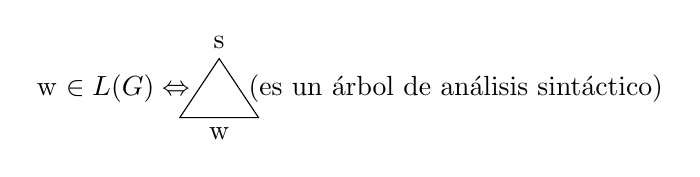
\begin{tikzpicture}
        \draw (0,0) node{}
          -- node[below]{w} (1,0) node{}
          -- node[right]{(es un árbol de análisis sintáctico)} (.5,.75) node[anchor=south]{s}
          -- node[left]{w $\in L(G) \Leftrightarrow$} cycle;
      \end{tikzpicture}

      \par
      \textbf{e.g.}\\
      \begin{center}
        \begin{minipage}{.2\textwidth}
          N $\rightarrow$ B\\
          N $\rightarrow$ NB\\
          B $\rightarrow$ 0\\
          B $\rightarrow$ 1
        \end{minipage}%
        \begin{minipage}{.3\textwidth}
          \begin{tikzpicture}
            \node[rectangle] (t1) {N};
            \node[rectangle, below left =.5 of t1] (t2) {N};
            \node[rectangle, below right =.5 of t1] (t3) {B};
            \node[rectangle, below left =.5 of t2] (t4) {N};
            \node[rectangle, below right =.5 of t2] (t5) {B};
            \node[rectangle, below =.5 of t3] (t6) {0};
            \node[rectangle, below =.5 of t4] (t7) {B};
            \node[rectangle, below =.5 of t5] (t8) {1};
            \node[rectangle, below =.5 of t7] (t9) {0};

            \path[thick]
              (t1.south) edge (t2)
                          edge (t3)
              (t2.south) edge (t4)
                          edge (t5)
              (t3.south) edge (t6)
              (t4.south) edge (t7)
              (t5.south) edge (t8)
              (t7.south) edge (t9);
          \end{tikzpicture}
        \end{minipage}%
        \begin{minipage}{.4\textwidth}
          \raggedright
          Cada nodo es equivalente a un array en el que se referencian sus hijos en orden.
        \end{minipage}
      \end{center}

  \section{Especificación sintáctica}
    \subsection{Determinar las clases sintácticas}
      \par
      ¿Cómo? A partir de la especificación informal.

      \bigskip
      \par
      De arriba a abajo:
      \begin{itemize}
        \item Identificar las clases complejas.
        \item Descomponerlas en clases más simples hasta llegar a las clases léxicas.
      \end{itemize}

      \bigskip
      \par
      Descomposición $\rightarrow$ Las clases resultantes deben estar al mismo nivel, el más alto posible.

      \bigskip
      \par
      \textbf{e.g.} L que describe libros
      \begin{center}
        \begin{minipage}{.4 \textwidth}
          \hspace*{5mm}Titulo [...]\\
          \hspace*{5mm}Autores [Autor]...[Autor]\\
          \hspace*{5mm}Capitulo [...][...]\\
          \hspace*{5mm}...\\
          \hspace*{5mm}Capitulo [...][...]
        \end{minipage}%
        \begin{minipage}{.5 \textwidth}
          \begin{tikzpicture}
            \node[rectangle] (lib) {Libro};
            \node[rectangle, below left =.8 of lib] (cab) {Cabecera};
            \node[rectangle, below right =.8 of lib] (cuer) {Cuerpo};
            \node[rectangle, below left =.5 of cab] (tit) {Titulo};
            \node[rectangle, below right =.5 of cab] (auts) {Autores};
            \node[rectangle, below =.5 of cuer] (cap) {Capitulo};
            \node[rectangle, below =.5 of auts] (aut) {Autor};
            \node[rectangle, below=.5 of cap] (tcap) {TituloCap};
            \node[rectangle, right=.5 of tcap] (ccap) {ContenidoCap};

            \path[thick]
              (lib.south) edge (cab)
                          edge (cuer)
              (cab.south) edge (tit)
                          edge (auts)
              (cuer.south) edge (cap)
              (auts.south) edge (aut)
              (cap.south) edge (tcap)
                          edge (ccap);
          \end{tikzpicture}
          \captionof{figure}{Árbol informal.}
        \end{minipage}
        \begin{minipage}{.4 \textwidth}
          \hspace*{5mm}Clases léxicas\\
          \hspace*{10mm}Autores\\
          \hspace*{10mm}Capitulo\\
          \hspace*{10mm}CAP\\
          \hspace*{10mm}CCIE\\
          \hspace*{10mm}Texto
        \end{minipage}%
        \begin{minipage}{.5 \textwidth}
          \vspace{10mm}
          \begin{tikzpicture}
            \node[rectangle, draw=black] (lib) {Libro};
            \node[rectangle, draw=black, below left =.8 of lib] (cab) {Cabecera};
            \node[rectangle, draw=black, below right =.8 of lib] (cuer) {Cuerpo};
            \node[rectangle, draw=black, below left =.6 and .5 of cab] (tit) {Title};
            \node[rectangle, draw=black, below right =.6 and .5 of cab] (auts) {Authors};
            \node[rectangle, draw=black, below =.5 of cuer] (cap) {Chapter};
            \node[rectangle, draw=black, below=.5 of cap] (tcap) {CTitle};
            \node[rectangle, draw=black, right=.5 of tcap] (ccap) {CContent};
            \node[rectangle, draw=black, below left=1.2 and 0 of tcap] (blo) {Bloque};
            \node[rectangle, draw=black, below =.5of blo] (tex) {Texto};

            \path[thick, ->]
              (lib.south) edge (cab)
                          edge (cuer)
              (cab.south) edge (tit)
                          edge (auts)
              (cuer.south) edge (cap)
              (tit.south) edge (blo)
              (auts.south) edge node[right, very near start] {+} (blo)
              (cap.south) edge (tcap)
                          edge (ccap)
              (tcap.south) edge (blo)
              (ccap.south) edge (blo)
              (blo.south) edge node[right] {$\ast$} (tex);
          \end{tikzpicture}
          \captionof{figure}{Árbol formal.}
        \end{minipage}
      \end{center}

    \subsection{Patrones para secuencias}
      \begin{itemize}
        \item Secuencia de 1 o más $I_s$, separados por $\Box$.\\
            \hspace{3mm}\textbf{e.g.} I $\mid$ I $\Box$ I $\mid$ I $\Box$ I $\Box$ I...\\
            \vspace{2mm}
            \hspace{3mm}LI $\rightarrow$ I\\
            \hspace{3mm}LI $\rightarrow$ LI $\Box$ I\\
            \vspace{2mm}
            \hspace{3mm}\textbf{e.g.}\\
            \hspace{3mm}NUM $\rightarrow$ B\\
            \hspace{3mm}NUM $\rightarrow$ NUM , B
        \item Secuencia de 0 o más $I_s$, separados por $\Box$.\\
            \hspace{3mm}S $\rightarrow$ $\varepsilon$\\
            \hspace{3mm}S $\rightarrow$ LI\\
            \hspace{3mm}LI $\rightarrow$ I\\
            \hspace{3mm}LI $\rightarrow$ LI $\Box$ I\\
            \vspace{2mm}
            \hspace{3mm}\textbf{e.g.} Declaraciones\\
            \hspace{3mm}Decs $\rightarrow$ $\varepsilon$\\
            \hspace{3mm}Decs $\rightarrow$ LDEC\\
            \hspace{3mm}LDEC $\rightarrow$ Dec\\
            \hspace{3mm}LDEC $\rightarrow$ LDEC ; Dec
      \end{itemize}

      \par
      Como caso particular de los patrones anteriores tenemos aquellos en que $\Box$ es
      $\varepsilon$, no están separados por nada.
      \begin{itemize}
        \item Secuencia de 1 o más $I_s$.\\
            \hspace{3mm}LI $\rightarrow$ I\\
            \hspace{3mm}LI $\rightarrow$ LI I
        \item Secuencia de 0 o más $I_s$.\\
            \hspace{3mm}S $\rightarrow$ $\varepsilon$\\
            \hspace{3mm}S $\rightarrow$ LI\\
            \hspace{3mm}LI $\rightarrow$ I\\
            \hspace{3mm}LI $\rightarrow$ LI I
      \end{itemize}

      \par
      También es posible usar un terminador en lugar de un separador para cada item.\\
      \hspace{3mm}\textbf{e.g.} \underline{I $\Box$} \underline{I $\Box$} \underline{I $\Box$}...
        donde I $\Box$ es un item.\\
      \begin{itemize}
        \item Secuencia de 1 o más $I_s$ terminados en $\Box$.\\
            \hspace{3mm}LI $\rightarrow$ BI\\
            \hspace{3mm}LI $\rightarrow$ LI BI\\
            \hspace{3mm}BI $\rightarrow$ I $\Box$\\
        \item Secuencia de 0 o más $I_s$ terminados en $\Box$.\\
            \hspace{3mm}S $\rightarrow$ $\varepsilon$\\
            \hspace{3mm}S $\rightarrow$ LI\\
            \hspace{3mm}LI $\rightarrow$ BI\\
            \hspace{3mm}LI $\rightarrow$ LI BI\\
            \hspace{3mm}BI $\rightarrow$ I $\Box$\\
      \end{itemize}

      \par
      \textbf{e.g.} Libro\\
      \begin{center}
        \begin{minipage}{.5\textwidth}
          \hspace*{5mm}Libro $\rightarrow$ Cabecera Cuerpo\\
          \hspace*{5mm}Cabecera $\rightarrow$ Title Authors\\
          \hspace*{5mm}Title $\rightarrow$ \underline{Titulo} Bloque\\
          \hspace*{5mm}Authors $\rightarrow$ \underline{Autores} LBloques\\
          \hspace*{5mm}LBloques $\rightarrow$ Bloque\\
          \hspace*{5mm}LBloques $\rightarrow$ LBloques Bloque\\
          \hspace*{5mm}Cuerpo $\rightarrow$ LChapter\\
          \hspace*{5mm}LChapter $\rightarrow$ Chapter\\
          \hspace*{5mm}LChapter $\rightarrow$ LChapter Chapter\\
        \end{minipage}%
        \begin{minipage}{.5\textwidth}
          \hspace*{5mm}Chapter $\rightarrow$ CTitle CContent\\
          \hspace*{5mm}CTitle $\rightarrow$ \underline{Capitulo} Bloque\\
          \hspace*{5mm}CContent $\rightarrow$ Bloque\\
          \hspace*{5mm}Bloque $\rightarrow$ $[$CTexto$]$\\
          \hspace*{5mm}CTexto $\rightarrow$ $\varepsilon$\\
          \hspace*{5mm}CTexto $\rightarrow$ LTexto\\
          \hspace*{5mm}LTexto $\rightarrow$ Texto\\
          \hspace*{5mm}LTexto $\rightarrow$ LTexto Texto\\
        \end{minipage}
      \end{center}

    \subsection{Patrones para operadores}
      \par
      La prioridad indica el orden en que los operadores se evaluan, si dos tienen la misma
      prioridad se consulta la asociatividad, a izquierdas o a derechas.\\
      \hspace{3mm}\textbf{e.g.}\\
      \begin{center}
        \begin{minipage}{.3\textwidth}
          \hspace{10mm}\underline{\underline{\underline{5 + 6} $-$ \underline{7 $\ast$ 8}} + 9}
        \end{minipage}%
        \begin{minipage}{.7\textwidth}
          $\ast$ es el más prioritario.\\
          + y - son igual de prioritarios pero asocian a izquierdas.
        \end{minipage}
      \end{center}

      \par
      Cada operador tiene un nivel de prioridad, pueden existir multiples operadores con un mismo
      nivel.
      \begin{itemize}
        \item Operadores binarios infijos.\\
          \hspace{3mm}Pueden asociar a izquierdas\\
          \hspace{5mm}\textbf{e.g.} \underline{\underline{5 + 6} + 7}\\
          \vspace{2mm}
          \hspace{3mm}O a derechas.\\
          \hspace{5mm}\textbf{e.g.} \underline{5 + \underline{6 + 7}}\\
          \vspace{2mm}
          \hspace{3mm}O no asociar, no está permitido encadenar operadores.\\
          \hspace{5mm}\textbf{e.g.} {\color{red}5 + 6 + 7}
        \item Operadores unarios prefijos.\\
          \hspace{3mm}\textbf{e.g.} -5\\
          \vspace{2mm}
          Pueden ser...
          \begin{itemize}
            \item ...\textbf{asociativos}, pueden encadenarse varios.
            \item ...\textbf{no asociativos}, no pueden encadenarse.
          \end{itemize}
          Asocian siempre a derechas.
        \item Operadores unarios postfijos.\\
          \hspace{3mm}\textbf{e.g.} 5+, x++\\
          \vspace{2mm}
            Pueden ser...
            \begin{itemize}
              \item ...\textbf{asociativos}, pueden encadenarse varios.
              \item ...\textbf{no asociativos}, no pueden encadenarse.
            \end{itemize}
            Asocian siempre a izquierdas.
      \end{itemize}

      \par
      \textbf{e.g.} Lenguaje\\
      \begin{center}
        \begin{minipage}{.35\textwidth}
          \begin{itemize}
            \item Numeros y variables.
            \item +, $-$, $\ast$, /, $-$ unario.
          \end{itemize}
        \end{minipage}%
        \begin{minipage}{.65\textwidth}
          \begin{tabular}{||c c c c c||}
            \hline
            Operador & Aridad & Tipo & Prioridad & Asociatividad \\ [0.5ex]
            \hline\hline
            +,$-$ & 2 &  & 0 & izquierda \\
            \hline
            *,/ & 2 &  & 1 & izquierda \\
            \hline
            $-$ & 1 & prefijo & 2 & si \\ [1ex]
            \hline
          \end{tabular}
        \end{minipage}
        \begin{minipage}{.5\textwidth}
          \vspace{5mm}
          \underline{\underline{\underline{5 + 6} $-$ \underline{\underline{$-$7} $\ast$ 8}} + 9}
        \end{minipage}
      \end{center}

      \par
      Si existen varios operadores con la misma prioridad pero que asocian distinto porque existen
      multiples interpretaciones.
      \begin{center}
        \begin{minipage}{.65\textwidth}
          \begin{tabular}{||c c c c c||}
            \hline
            Operador & Aridad & Tipo & Prioridad & Asociatividad \\ [0.5ex]
            \hline\hline
            + & 2 &  & 0 & izquierda \\
            \hline
            $-$ & 2 &  & 0 & derecha \\
            \hline
            *,/ & 2 &  & 1 & izquierda \\
            \hline
            $-$ & 1 & prefijo & 2 & si \\ [1ex]
            \hline
          \end{tabular}
        \end{minipage}%
        \begin{minipage}{.35\textwidth}
          \hspace*{10mm}\underline{5 + \underline{6 + 7}}\\\\
          \hspace*{10mm}\underline{\underline{5 + 6} + 7}
        \end{minipage}
      \end{center}

      \begin{center}
        \begin{minipage}{.5\textwidth}
          \hspace*{3mm}Exp $\rightarrow$ Variable\\
          \hspace*{3mm}Exp $\rightarrow$ Numero\\
          \hspace*{3mm}Exp $\rightarrow$ OpUn Exp\\
          \hspace*{3mm}Exp $\rightarrow$ Exp OpBin Exp\\
          \hspace*{3mm}OpUn $\rightarrow$ $-$\\
          \hspace*{3mm}OpBin $\rightarrow$ +\\
          \hspace*{3mm}OpBin $\rightarrow$ $-$\\
          \hspace*{3mm}OpBin $\rightarrow$ $\ast$\\
          \hspace*{3mm}OpBin $\rightarrow$ /
        \end{minipage}%
        \begin{minipage}{.5\textwidth}
          \par
          \textit{Num + Num + Num}\\
          \begin{tikzpicture}
            \node[rectangle] (e1) {Exp};
            \node[rectangle, below left =.5 of e1] (e2) {Exp};
            \node[rectangle, below =.4 of e1] (ob1) {OpBin};
            \node[rectangle, below right =.5 of e1] (e3) {Exp};
            \node[rectangle, below left =.5 and 1.5 of e2] (e4) {Exp};
            \node[rectangle, below left=.5 and .2 of e2] (ob2) {OpBin};
            \node[rectangle, below left =.5 and -.7 of e2] (e5) {Exp};

            \node[rectangle, below = .5 of e3] (v1) {Num};
            \node[rectangle, below = .5 of e4] (v2) {Num};
            \node[rectangle, below = .5 of e5] (v3) {Num};
            \node[rectangle, below = .5 of ob1] (o1) {+};
            \node[rectangle, below = .5 of ob2] (o2) {+};

            \path[thick]
              (e1.south) edge (e2)
                          edge (ob1)
                          edge (e3)
              (e2.south) edge (e4)
                          edge (ob2)
                          edge (e5)
              (e3.south) edge (v1)
              (e4.south) edge (v2)
              (e5.south) edge (v3)
              (ob1.south) edge (o1)
              (ob2.south) edge (o2);
          \end{tikzpicture}
        \end{minipage}
        \begin{minipage}{.5\textwidth}
          \raggedright
          \par
          Como hemos encontrado dos posibles árboles de derivación la gramática es ambigua y no vale.
        \end{minipage}%
        \begin{minipage}{.5\textwidth}
          \begin{tikzpicture}
            \node[rectangle] (e1) {Exp};
            \node[rectangle, below left =.5 of e1] (e2) {Exp};
            \node[rectangle, below =.4 of e1] (ob1) {OpBin};
            \node[rectangle, below right =.5 of e1] (e3) {Exp};
            \node[rectangle, below right =.5 and 1.5 of e3] (e4) {Exp};
            \node[rectangle, below right=.5 and .2 of e3] (ob2) {OpBin};
            \node[rectangle, below right =.5 and -.7 of e3] (e5) {Exp};

            \node[rectangle, below = .5 of e2] (v1) {Num};
            \node[rectangle, below = .5 of e4] (v2) {Num};
            \node[rectangle, below = .5 of e5] (v3) {Num};
            \node[rectangle, below = .5 of ob1] (o1) {+};
            \node[rectangle, below = .5 of ob2] (o2) {+};

            \path[thick]
              (e1.south) edge (e2)
                          edge (ob1)
                          edge (e3)
              (e3.south) edge (e4)
                          edge (ob2)
                          edge (e5)
              (e2.south) edge (v1)
              (e4.south) edge (v2)
              (e5.south) edge (v3)
              (ob1.south) edge (o1)
              (ob2.south) edge (o2);
          \end{tikzpicture}
        \end{minipage}
      \end{center}

      \par
      Cada nivel de prioridad tendrá su propio terminal.\\
      Si crece a izquierdas reduzco el nivel de prioridad de la derecha, si es a derechas baja el
      de la izquierda y si no asocia ambos aumentan.

      \begin{center}
        \begin{minipage}{.5\textwidth}
          \hspace*{3mm}Exp0 $\rightarrow$ Exp0 OpBin0 Exp1\\
          \hspace*{3mm}Exp0 $\rightarrow$ Exp1\\
          \hspace*{3mm}Exp1 $\rightarrow$ Exp1 OpBin1 Exp2\\
          \hspace*{3mm}Exp1 $\rightarrow$ Exp2\\
          \hspace*{3mm}Exp2 $\rightarrow$ Exp2 OpBin2 Exp3\\
          \hspace*{3mm}Exp2 $\rightarrow$ Exp3\\
          \hspace*{3mm}Exp3 $\rightarrow$ (Exp0)\\
          \hspace*{3mm}Exp3 $\rightarrow$ Num\\
          \hspace*{3mm}Exp3 $\rightarrow$ Var\\
          \hspace*{3mm}OpBin0 $\rightarrow$ +\\
          \hspace*{3mm}OpBin0 $\rightarrow$ $-$\\
          \hspace*{3mm}OpBin1 $\rightarrow$ $\ast$\\
          \hspace*{3mm}OpBin1 $\rightarrow$ /\\
          \hspace*{3mm}OpUn2 $\rightarrow$ $-$
        \end{minipage}%
        \begin{minipage}{.5\textwidth}
          \par
          \textit{Num + Num + Num}\\
          \begin{tikzpicture}
            \node[rectangle] (e1) {Exp0};
            \node[rectangle, below left =.5 of e1] (e2) {Exp0};
            \node[rectangle, below =.4 of e1] (ob1) {OpBin0};
            \node[rectangle, below right =.5 of e1] (e3) {Exp1};
            \node[rectangle, below left =.5 and 1.7 of e2] (e4) {Exp0};
            \node[rectangle, below left=.5 and .1 of e2] (ob2) {OpBin0};
            \node[rectangle, below left =.5 and -1 of e2] (e5) {Exp1};

            \node[rectangle, below = .5 of e3] (e31) {Exp1};
            \node[rectangle, below = .5 of e31] (e32) {Exp2};
            \node[rectangle, below = .5 of e32] (e33) {Exp3};
            \node[rectangle, below = .5 of e33] (v1) {Num};

            \node[rectangle, below = .5 of e4] (e41) {Exp1};
            \node[rectangle, below = .5 of e41] (e42) {Exp2};
            \node[rectangle, below = .5 of e42] (e43) {Exp3};
            \node[rectangle, below = .5 of e43] (v2) {Num};

            \node[rectangle, below = .5 of e5] (e51) {Exp1};
            \node[rectangle, below = .5 of e51] (e52) {Exp2};
            \node[rectangle, below = .5 of e52] (e53) {Exp3};
            \node[rectangle, below = .5 of e53] (v3) {Num};

            \node[rectangle, below = .5 of ob1] (o1) {+};
            \node[rectangle, below = .5 of ob2] (o2) {+};

            \path[thick]
              (e1.south) edge (e2)
                          edge (ob1)
                          edge (e3)
              (e2.south) edge (e4)
                          edge (ob2)
                          edge (e5)
              (e3.south) edge (e31)
              (e31.south) edge (e32)
              (e32.south) edge (e33)
              (e33.south) edge (v1)
              (e4.south) edge (e41)
              (e41.south) edge (e42)
              (e42.south) edge (e43)
              (e43.south) edge (v2)
              (e5.south) edge (e51)
              (e51.south) edge (e52)
              (e52.south) edge (e53)
              (e53.south) edge (v3)
              (ob1.south) edge (o1)
              (ob2.south) edge (o2);
          \end{tikzpicture}
        \end{minipage}
        \begin{minipage}{.5\textwidth}
          \vspace{5mm}
          \par
          \textit{Num + (Num + Num)}\\
          \begin{tikzpicture}
            \node[rectangle] (e1) {Exp0};
            \node[rectangle, below left =.5 of e1] (e2) {Exp0};
            \node[rectangle, below =.4 of e1] (ob1) {OpBin0};
            \node[rectangle, below right =.5 of e1] (e3) {Exp1};
            \node[rectangle, below =.5 of e3] (e32) {Exp2};
            \node[rectangle, below =.5 of e32] (e33) {Exp3};
            \node[rectangle, below right =.5 and -1 of e33] (PAP) {(};
            \node[rectangle, below right=.5 and .1 of e33] (e30) {Exp0};
            \node[rectangle, below right =.5 and 1.7 of e33] (PCI) {)};
            \node[rectangle, below left =.5 of e30] (e4) {Exp1};
            \node[rectangle, below =.4 of e30] (ob2) {OpBin0};
            \node[rectangle, below right =.5 of e30] (e5) {Exp0};

            \node[rectangle, below = .5 of e2] (e21) {Exp1};
            \node[rectangle, below = .5 of e21] (e22) {Exp2};
            \node[rectangle, below = .5 of e22] (e23) {Exp3};
            \node[rectangle, below = .5 of e23] (v1) {Num};

            \node[rectangle, below = .5 of e4] (e41) {Exp1};
            \node[rectangle, below = .5 of e41] (e42) {Exp2};
            \node[rectangle, below = .5 of e42] (e43) {Exp3};
            \node[rectangle, below = .5 of e43] (v2) {Num};

            \node[rectangle, below = .5 of e5] (e51) {Exp1};
            \node[rectangle, below = .5 of e51] (e52) {Exp2};
            \node[rectangle, below = .5 of e52] (e53) {Exp3};
            \node[rectangle, below = .5 of e53] (v3) {Num};

            \node[rectangle, below = .5 of ob1] (o1) {+};
            \node[rectangle, below = .5 of ob2] (o2) {+};

            \path[thick]
              (e1.south) edge (e2)
                          edge (ob1)
                          edge (e3)
              (e3.south) edge (e32)
              (e32.south) edge (e33)
              (e33.south) edge (e30)
                          edge (PAP)
                          edge (PCI)
              (e30.south) edge (e4)
                          edge (ob2)
                          edge (e5)
              (e2.south) edge (e21)
              (e21.south) edge (e22)
              (e22.south) edge (e23)
              (e23.south) edge (v1)
              (e4.south) edge (e41)
              (e41.south) edge (e42)
              (e42.south) edge (e43)
              (e43.south) edge (v2)
              (e5.south) edge (e51)
              (e51.south) edge (e52)
              (e52.south) edge (e53)
              (e53.south) edge (v3)
              (ob1.south) edge (o1)
              (ob2.south) edge (o2);
          \end{tikzpicture}
        \end{minipage}%
        \begin{minipage}{.5\textwidth}
          \par
          El árbol de la izquierda sería equivalente al siguiente.\\
          \begin{tikzpicture}
            \node[rectangle] (o1) {+};
            \node[rectangle, below left =.5 of o1] (n1) {Num};
            \node[rectangle, below right=.5 of o1] (o2) {+};
            \node[rectangle, below left =.5 of o2] (n2) {Num};
            \node[rectangle, below right =.5 of o2] (n3) {Num};

            \path[thick]
              (o1.south) edge (n1)
                          edge (o2)
              (o2.south) edge (n2)
                          edge (n3);
          \end{tikzpicture}
        \end{minipage}

        \begin{minipage}{\textwidth}
          \par
          \textit{Num $-$ Num $\ast$ $-$Num + Num}\\
          \centering
          \vspace{2mm}
          \begin{tikzpicture}
            \node[rectangle] (e1) {Exp0};

            \node[rectangle, below =.5 of e1] (ob1) {OpBin0};
            \node[rectangle, left = 3 of ob1] (e2) {Exp0};
            \node[rectangle, right = 3 of ob1] (e3) {Exp1};

            \node[rectangle, below =.5 of e2] (ob2) {OpBin0};
            \node[rectangle, left = of ob2] (e4) {Exp0};
            \node[rectangle, right = of ob2] (e5) {Exp1};

            \node[rectangle, below =.5 of e4] (e41) {Exp1};
            \node[rectangle, below =.5 of e41] (e42) {Exp2};
            \node[rectangle, below =.5 of e42] (e43) {Exp3};
            \node[rectangle, below =.5 of e43] (ve43) {Num};

            \node[rectangle, below =.5 of ob2] (vob2) {+};

            \node[rectangle, below =.5 of e5] (e6) {Exp1};
            \node[rectangle, right = of e6] (ob3) {OpBin1};
            \node[rectangle, right = of ob3] (e7) {Exp2};

            \node[rectangle, below =.5 of e6] (e62) {Exp2};
            \node[rectangle, below =.5 of e62] (e63) {Exp3};
            \node[rectangle, below =.5 of e63] (ve63) {Num};

            \node[rectangle, below left=.5 and -.2 of ob3] (vob3) {$\ast$};

            \node[rectangle, below =.5 of e7] (e8) {Exp2};
            \node[rectangle, left =.3 of e8] (oun1) {OpUn2};

            \node[rectangle, below =.5 of oun1] (voun1) {$-$};

            \node[rectangle, below =.5 of e8] (e83) {Exp3};
            \node[rectangle, below =.5 of e83] (ve83) {Num};

            \node[rectangle, below =.5 of ob1] (vob1) {+};

            \node[rectangle, below =.5 of e3] (e32) {Exp2};
            \node[rectangle, below =.5 of e32] (e33) {Exp3};
            \node[rectangle, below =.5 of e33] (ve33) {Num};

            \path[thick]
              (e1.south) edge (e2)
                          edge (ob1)
                          edge (e3)
              (e2.south) edge (e4)
                          edge (ob2)
                          edge (e5)
              (e4.south) edge (e41)
              (e41.south) edge (e42)
              (e42.south) edge (e43)
              (e43.south) edge (ve43)
              (ob2.south) edge (vob2)
              (e5.south) edge (e6)
                          edge (ob3)
                          edge (e7)
              (e6.south) edge (e62)
              (e62.south) edge (e63)
              (e63.south) edge (ve63)
              (ob3.south) edge (vob3)
              (e7.south) edge (oun1)
                          edge (e8)
              (oun1.south) edge (voun1)
              (e8.south) edge (e83)
              (e83.south) edge (ve83)
              (ob1.south) edge (vob1)
              (e3.south) edge (e32)
              (e32.south) edge (e33)
              (e33.south) edge (ve33);
          \end{tikzpicture}
        \end{minipage}
      \end{center}
\end{document}